\documentclass[a4paper]{article}
\usepackage[utf8]{inputenc}
\usepackage[T1]{fontenc}
\usepackage[pdftex]{graphicx}
\usepackage{fancyhdr}
\usepackage{lscape}
\usepackage{color}
\usepackage{qtree}
\usepackage[english]{babel}
\usepackage{graphicx}
\usepackage[colorinlistoftodos]{todonotes}
\usepackage{listings}
\usepackage{color}
\usepackage{changepage}
\usepackage[margin=1in]{geometry}
\definecolor{codegreen}{rgb}{0,0.6,0}
\definecolor{codegray}{rgb}{0.5,0.5,0.5}
\definecolor{codepurple}{rgb}{0.58,0,0.82}
\definecolor{backcolour}{rgb}{0.95,0.95,0.92}
\usepackage[parfill]{parskip}

 \lstdefinestyle{mystyle}{
 	backgroundcolor=\color{backcolour},   
 	commentstyle=\color{codegreen},
 	keywordstyle=\color{magenta},
 	numberstyle=\tiny\color{codegray},
 	stringstyle=\color{codepurple},
 	basicstyle=\footnotesize,
 	breakatwhitespace=false,         
 	breaklines=true,                 
 	captionpos=b,                    
 	keepspaces=true,                 
 	numbers=left,                    
 	numbersep=5pt,                  
 	showspaces=false,                
 	showstringspaces=false,
 	showtabs=false,                  
 	tabsize=2
 }
 
\lstset{
	style=mystyle,
	inputencoding=utf8,
	extendedchars=true,
	literate={á}{{\'a}}1 {ã}{{\~a}}1 {é}{{\'e}}1,
	escapechar=\&
}
\title{Algorithmique et structures de données : Mission 2}
\date{18 octobre 2014}
\author{Groupe 1.2: Ivan Ahad - Jérôme Bertaux - Rodolphe Cambier \\ 
	Baptiste Degryse - Wojciech Grynczel - Charles Jaquet}



\begin{document}
\maketitle



\paragraph{Question 1 (Bertaux Jérôme)}
Les trois méthodes principales du type abstrait Map sont :
\begin{itemize}
\item get(k) : Permet de récupérer la valeur associé à la clef k et si aucune valeur n'est associé à cette clef on récupère un null.
\item put(k,v) : Si aucune entrée n'est associé à la clef k alors cette entrée est ajouté et on retourne null. Sinon on remplace l'ancienne valeur de k par la nouvelle et on retourne l'ancienne valeur.
\item remove(k) : Retire l'entrée associé à la clef k et retourne sa valeur et si aucune entrée n'est associé à k alors on retourne null.
\end{itemize}
Dans ce contexte :
\begin{itemize}
\item clef : Une clef est un identifiant unique qui permet d'identifier une valeur dans la Map. 
\item valeur : Une valeur est l'objet de donnée qu'on souhaite sotcker dans la Map.
\item \textit{entry} : Une \textit{entry} est une  pair clef-valeur.
\end{itemize}
Il est possible d'insérer une entrée k-null dans une Map. Donc quand on demande la valeur de la clef k on récupère un null non pas car il n'existe pas dans la Map mais parce que cette valeur est autorisée. Certaines implémentations de Map interdisent l'utilisation de valeur null. Mais pour lever l'ambiguité dans les implémentations autorisant la valeur null, il existe une méthode containsKey(k) pour vérifier si k est une clef valide.
Voici quelques exemples d'application d'un Map :
\begin{itemize}
\item Dans un annuaire téléphonique : la clef est le numéro de téléphone et la valeur est le nom de la personne.
\item Dans le registre national : la clef est le numéro d'identification du registre national et la valeur est le dossier personnel du citoyen.
\item Dans une banque : la clef est le numéro de compte de la personne et la valeur est le dossier bancaire de la personne.
\end{itemize}

\paragraph{Question 2 (Bertaux Jérôme)}
\begin{enumerate}
\item Une hashtable : Les opérations basiques de la Map get, put et remove peuvent être implémenter en O(1).
\item Une table de recherche ordonnée : son espace nécessaire est de O(n). Le get s'exécute en O(log n), le put en O(n) et le remove en O(n).
\item Une liste non ordonnée : Les méthodes fondamentales s'exécute en O(n) dans les pires cas car il faut parcourir toute la liste pour vérifier l'existance d'une entrée déjà existante.
\item Une Skip List est une implémentation possible pour un dictionnaire non ordonné mais il n'est pas judicieux de l'utiliser. Car le système de rangement des entrées est basé sur de l'aléatoire. Donc la recherche se fait en O(log n), l'insertion en O(log n) et la suppresion en O(log n).
\end{enumerate}

\paragraph{Q3 (Baptiste Degryse)}
Il faut utiliser l'algorithme de binary search qui est de complexité O(log(n)). Il faut l'appliquer sur chaque ligne du tableau, multipliant cette complexité par n. L'algorithme est le suivant:
\begin{lstlisting}[language=Java]
int [] lastOne=new int[n];
for(z=0;z<n;z++){
	int a=0,b=n,lastOne;
	while(b-a>1){
		if(tab[z][(a+b)/2]==0)
			b=(a+b)/2;
		else if(tab[z][(a+b)/2]==1)
			a=(a+b)/2;
	}
	lastOne[z]=a;
}

\end{lstlisting}

\paragraph{Q4 (Baptiste Degryse)}
Une specification de la méthode union:
\begin{lstlisting}[language=Java]
/**
* @input : d1 et d2, deux dictionnaires ordonnés
* @output : un dictionnaire ordonné contenant l'union des éléments des deux dictionnaires passés en entrée.
*/
\end{lstlisting}
Pour l'algorithme, dans le cas d'une implémentation des dictionnaires en tables ordonnée:
\begin{lstlisting}[language=Java]
Entree tab[]= new Entree [d1.size()+d2.size()]
int i,j;
while(i+j<tab.size()){
	if( i>d1.size() || (j<d2.size() && d1[i].key()>d2[j].key())){
		tab[i+j]=d2[j];
		j++;
	}
	else{
		tab[i+j]=d1[i];
		i++;
	}
}
return tab;
\end{lstlisting}
Dans le cas de l'utilisation d'une table de hachage, chaque appel dx[y] deviendrait dx[h(y)].

\paragraph{Q5}

\paragraph{Q6}

\paragraph{Q7 (Ivan)}

\paragraph*{Pouvez-vous déterminer précisément de quelle variante de table de hachage la classe Java.util.Hashtable s'agit?}

La classe java.util.Hashtable est une AbstractHashMap. 

\paragraph{Java fournit-il d'autres implémentations de l'interface Map? Faites un diagramme qui représente les interfaces et les classes qui se rapportent à map et précisez ce qui les caractérise.}
-Interface Map\\
-Classe AbstractMap : l'AbstractMap est un type abstrait de données qui représente une collection de paires clef-valeur et qui implémente l'interface Map.\\
-Classe UnsortedTableMap : La classe UnsortedTableMap étend la classe AbstractMap et correspond à une table dont les éléments de la collection ne sont pas ordonnés, ce qui implique un manque d'efficacité dû au fait que chaque méthode a une complexité linéaire au maximum au lieu d'être constante car il faut scanner tous les éléments pour trouver une entrée. \\
-Classe AbstractHashMap : La classe AbstractHashMap étend la classe AbstractMap. La principale différence est que les tables de hachages peuvent avoir des clés qui ne sont pas des entiers mais qui peuvent être des symboles.  \\ 
-Classe ChainHashMap : Cette classe étend la classe AbstractHashmap et utilise le chainage de sorte que toutes les valeurs ayant la même clef soient regroupés dans une structure chainée. Cela permet d'éviter les collisions.\\
-Classe ProbeHashMap : Cette classe étend la classe AbstractHashMap et utilise aussi un système permettant d'éviter les collisions. Le système est tel que si l'on veut insérer un élément dans la table mais qu'une clef possède déjà une valeur, on essaye d'insérer la valeur à la clef suivante, et ainsi de suite jusqu'à trouver une clef non-occupée. \\ 
\\
-Interface SortedMap : L'interface SortedMap étend l'interface Map. La particularité de SortedMap est que les valeurs sont mappés de sorte qu'ils soient ordonnés.\\
-Classe AbstractSortedMap : Il s'agit d'un type abstrait de données qui représente une collection ordonnée de paires clef-valeur. Cette classe implémente l'interface SortedMap.\\
-Classe SortedTableMap : Cette classe étend la classe AbstractSortedMap et correspond à une table dynamique dans laquelle sont stockées les entrées dans un ordre croissant selon la valeur des clefs. Grâce à cette structure la recherche binaire est possible.  \\
-Classe TreeMap : Cette classe permet de représenter les valeurs sous forme hiérarchique. \\ 

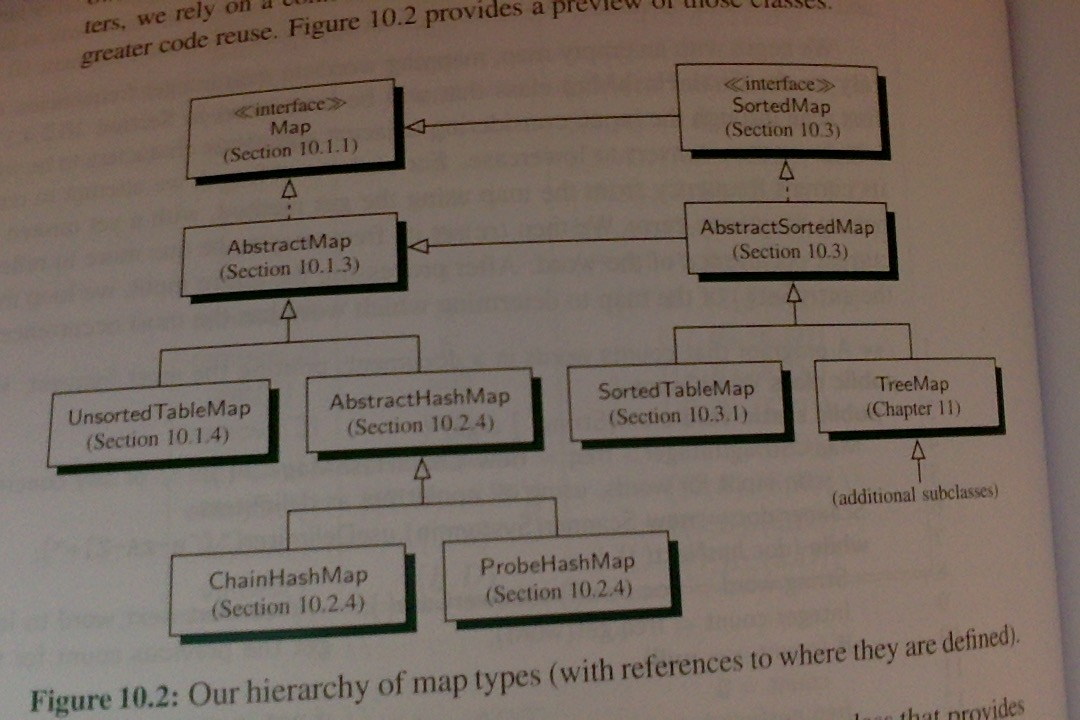
\includegraphics[scale=0.3]{diagramme.png}
\\
==> Diagramme représentant les classes et interfaces se rapportant à Map. \\
(Source : DSAJ6, page 374)\\

\paragraph{Qu'est-ce qui peut servir de clef pour une hashtable en Java?}
\paragraph*{}
Les chaines de caractères peuvent servir de clef en Java car il s'agit d'un type plus général que les caractères ou les entiers. Ainsi on peut utiliser plus de symboles pour définir les clefs. 

\paragraph{Q8 (Charles Jacquet)}
La question est de savoir comment faire pour implémenter la fonction remove(k) lorsqu'on utilise la technique du linear probing. Premièrement, le linéar probing signifie que lorsqu'on veut placer un élément, on en prend le hashcode, on le compresse. Ensuite, s'il y a une collision lors du placement dans la map, cette technique veut qu'on mette à l'élément à la position libre suivante. Voici les étapes à executer pour supprimer un élément:
\begin{itemize}
\item Chercher la position de l'élément grâce à la hashtable.
\item On le supprime
\item On crée une liste dans laquelle on met tous les éléments suivant jusqu'à ce qu'il y ait un élément vide.
\item On refait put(k) pour chaque élément pour être certain qu'ils soient au bon endroit.
\end{itemize}

Par contre, ici, la complexité varie, c'est-à-dire que dans le meilleur des cas, il y a un trou juste après l'élément, alors la complexité est en O(1). Par contre, dans le pire des cas, c'est-à-dire si l'élement à supprimer est le premier et que toute la map est remplie alors c'est en O(n).

\paragraph{Q9}



\end{document}